\subsection{User Experience}
 El sistema puede mostrar los datos de una forma precisa, optimizada, totalmente personaliza y ofrecerle
 la posibilidad al usuario de mejorar su vida considerablemente, sin embargo, si no proporcionamos una experiencia
 de usuario agradable y que reacciona a nuestras acciones, todos nuestros esfuerzos seran en vano.
 El usuario debe sentir que el sistema le ofrece la informacion de una manera fluida, limpia, intuitiva, directa y con
 una secuencia logica.\\
  
Esta secuencia le permitira al usuario la posibilidad de indagar por si mismo, como si la redaccion de una novela se tratara.

Buscamos simplicdad ya que el objetivo es representar la informacion, huiremos de toda decoracion innecesaria que emborrene
el objetivo principal. Recordemos que menos es mas. Un diseno complicado, con muchos colores y diferentes formas abstractas
sera mas dificil de interpretar por el usuario.

La representacion debe estar fuera de toda ambiguidad, no mostrar informacion que resulte enganosa o que haya que dedicar 
demasiado tiempo fijandonos en los detalles para poder interpretarla correctamente. Al representar la informacion sera 
incluido lo basicamente necesario, huyendo siempre de graficas recargadas que solo aporten ruido a la represetacion.

Buscaremos crear familiaridad, que el usuario pueda enterder de una forma rapida las estructuras utilizadas y 
le resulte facil de moverse con el minimo tiempo de aprendizaje posible. 

Ademas, en el mercado existen varios estandares a los que el usuario esta acostumbrado y sabe lo que esperar.
Por ejemplo una lupa, lo relacionamos con la accion de buscar, si utilizamos este icono, el usuario sabra rapidamente que
funcion realiza, sin embargo, si utilizamos uno completamente nuevo, puede incluso confundir al usuario\\

Es importante darle al usuario un grado de flexibilidad, que sea capaz de realizar sus propias selecciones para poder ver
los datos en los que esta interesando.

Cuando hablamos de fluidez, nos referimos a las interacciones usuario-sistema, es importante que las interacciones
sean como una conversacion a dos, donde uno pregunta y hace saber que esta escuchando y responde. Cuando el usuario 
requiere informacion del sistema, este performara un cambio que permita saber al usuario que ha recibido su accion y
con un tiempo de no mas de cinco segundos, debera de proporcionar una respuesta.

    
\subsubsection{How to solve it} 
Deberemos analizar con atencion que informacion queremos presentar y nos centraremos en este objetivo. Realizaremos un 
diseno limpio, donde todos los elementos sean facil de reconocer.
La estructura conllevara una secuencia logica, como si de una historia narrativa se tratara. 
Cada accion que el usuario pueda realizar, debera implementar una indicacion clara y ofrecer resultados en un 
periodo de menos de cinco segundos.
Huiremos de representaciones mas complicadas del nivel del usuario, intentaremos aplicar la familiaridad e intuitividad.
Es decir, si para la eleccion de fechas se utiliza un calendario, no tiene sentido utilizar un reloj de arena, esto confundira
mucho mas al usuario.
Ofrecer flexibilidad, el usuario debe ser capaz de interaccionar y elegir que quiere ver.

\subsubsection{How we solve it. Aire Guru} 
Nuestra herramienta utiliza una interpretacion de material design, el cual utiliza un diseno limpio, sin bordes ni decoraciones.
Se utiliza una gama de en tonos azules en combinacion con blanco y gris buscando un entorno relajado. 
Se ha cuidado que todos los textos tengan un nivel de contraste con su fondo, para que sea facil de leer.

Las graficas estan disenadas en 2D, ya que son mas faciles de interpretar y huimos de la ambiguedad que puede
proporcionar la profundidad como medida.


El workflow de las distintas secciones de Aire Guru esta detalladamente estudiada.
Aire Guru se comprende de distintas secciones. Mediante la seleccion de un punto en el mapa, nos
mostrara informacion detallada de este punto. A continuacion, cuenta con una seccion que filtrara la informacion acorde a las preferencias del usuario
y para concluir, muestra el historial de los contaminantes desde 2018 y el historial de la polucion al que el usuario ha estado
expuesto. 

Es de preveer que el usuario estara interesado en el nivel de polucion al que esta expuesto a tiempo real, por ello, para usuarios
que esten identificados y accedan a compartir su ubicacion, Aire Guru mostrara directeramente la polucion en el punto en el 
que se encuentra.
\begin{figure}[ht]
    \centering
    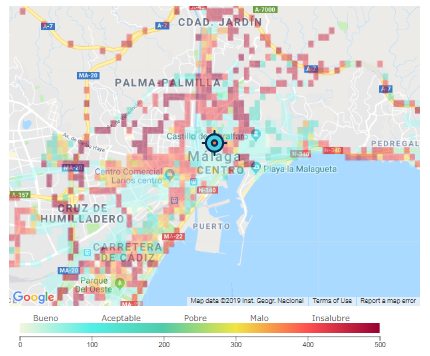
\includegraphics[width=12cm]{myLocation}
    \caption{My Location}
\end{figure}



Respecto a la flexibilidad, el usuario puede ver la situacion de la polucion del aire por fechas. El filtrado en la zona
intermedia, puede realizarse tanto por condiciones medicas como por agentes contamientes. Por ultimo, en zona inferior donde tenemos
los historicos por zona y personalizado, podemos visualizar la informacion con distinta granularidad, hora, dia, mes y ano y tambien podemos
seleccionar la fecha que deseamos.


\begin{figure}[ht]
    \centering
   \subfigure[Date filter]
    {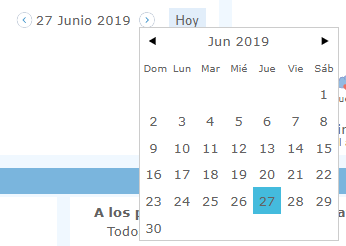
\includegraphics[width=5.5cm  ]{dateFilter}}
    \hfill
    \subfigure [Medical conditions filter]
       { \includegraphics[width=5.5cm]{MedicalConditionFilter}}
    \vfill
     \subfigure[Pollutans filter]
     { \centering 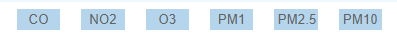
\includegraphics[width=6cm]{pollutansFilter}}
  
  \caption{Filters}
    \end{figure}


Se utiliza el mismo estilo, colores e iconografia en todo el diseno para que el usuario se familierize rapidamente y pueda
prestar atencion al significado de los datos en vez de perderse en el diseno e intentar encontrar su significado. 

Debido a la gran cantidad de datos que se le ofrece al usuario, se ha implementado una rueda de espera para indicar
que la herramienta esta procesando informacion. Cada vez que se pulsa un control en la pagina, se indica con un cambio
de tonalidad. Ademas se utilizan transiciones progresivas, cuando las graficas tienen que representar informacion nueva no lo hace 
de golpe, ya que esto podria producir un guino que puede ser interpretado como un error por parte del usuario.



\begin{figure}[ht]
    \centering

    \caption{Waiting symbol}
\end{figure}

\begin{figure}[ht]
    \centering
   \subfigure[Searching bar]
    {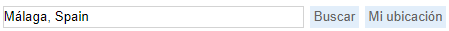
\includegraphics[width=5.5cm  ]{searchingBar}}
    \hfill
    \subfigure [Tabs]
       { 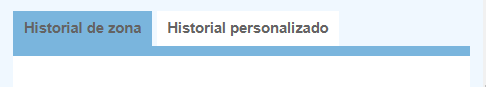
\includegraphics[width=5.5cm]{tabs}}
    \vfill
     \subfigure[Link]
     { 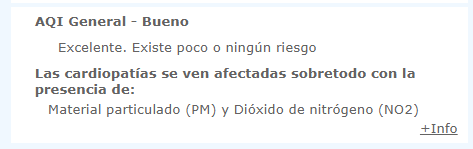
\includegraphics[width=6cm]{link}}
     \hfill
     \subfigure [Waiting symbol]
        { 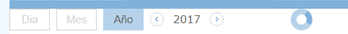
\includegraphics[width=5.5cm]{waitingSymbol}}
  
  \caption{Standard widgets}
    \end{figure}

    Los elementos que nos aportan familiaridad son la iconografia que utilizamos para mostrar el AQI. Utilizamos nubes, por representacion
    del aire, el entorno, se acompana de un corazon si la calidad es buena, de un simbolo de exclamacion si es pobre, de una cruz si es 
    mala y cambiamos a una mascara de gas si el estado es insalubre.
    
    Hoy en dia todos estamos acostumbrados a los mapas de GoogleMaps, por ello se ha integrado para representar el mapa y no otro,
    ya que los usuarios estan familiarizados por como se ven y en su manejo.
\elsparagraph{Evaluation}  
\begin{itemize}
    \done Tiene una estetica relajada donde prima las graficas con la informacion
    \done La representacion sigue una logica de secuencia
    \done Familiaridad, repeticion de estructuras y colores que representan lo mismo y estandares
    \done Flexibilidad. El usurio puede realizar multiples selecciones
    \crossed Los tiempos de espera se deberian mejorar
\end{itemize}
\newpage